\documentclass[slidestop,usepdftitle=false,10pt]{beamer}
\usepackage[accumulated]{beamerseminar}
\usepackage[english]{babel}
\usepackage{beamertexpower}
\usepackage{multicol}
\usepackage{beamerthemeshadow}
\usepackage[ansinew]{inputenc}
\usepackage{graphics}
\usepackage{graphicx}
\usepackage{color}
\usepackage{animate}
% \usepackage{movie15}
\usepackage{bibentry}
\usepackage{epstopdf}
\usepackage{media9}
%\usepackage{enumerate}
\usepackage{amssymb,amsmath,graphicx,tikz,movie15}
\usepackage[linesnumbered,lined,boxed,commentsnumbered,ruled]{algorithm2e}
\usepackage{hyperref}
\usepackage[mathscr]{eucal}
\usepackage{optidef}
\usepackage{multirow}


%\usetheme[height=0mm]{Rochester}
%\usepackage[spanish]{babel}
%\usepackage[utf8]{inputenc}
%\input adefin.tex
%\beamertemplatenavigationsymbolsempty
%\beamersetaveragebackground{white!90!red}
%**********************************************************
\newtheorem{defn}{Definition}[section]
\newtheorem{ej}{Example}[section]
\newtheorem{ejs}{Examples}[section]
\newtheorem{prop}{Proposition}[section]
\newtheorem{nota}{Notation}[section]
\newtheorem{thm}{Theorem}[section]
\newtheorem{cor}{Corollary}[section]
\newtheorem{rem}{Remark}[section]
\newtheorem{lem}{Lemma}[section]

\def \Proof{\noindent{\underline {Proof:}}}
\def\fra#1#2{\frac{ #1}{ #2}}
\renewcommand*{\baselinestretch}{1}

\def\fra#1#2{\frac{ #1}{ #2}}
%\def\fra#1#2{\frac{\displaystyle #1}{\displaystyle #2}}
%\renewcommand*{\baselinestretch}{1}

\def\fra#1#2{\frac{\displaystyle #1}{\displaystyle #2}}

%\newcommand{\fra}[2]{\displaystyle{\frac{#1}{#2}}}


\newcommand{\bi}{\mathbf{b}}
\newcommand{\ta}{\mathbf{t}}
\newcommand{\no}{\mathbf{n}}
\newcommand{\nor}{\mathbf{N}}
\newcommand{\sv}{\mathbf{S}}
\newcommand{\norm}[2]{|| #1 ||_{#2}}
\newcommand{\norma}[1]{|#1|}
\newcommand{\R}[1]{\mathbb{R}^#1}
\newcommand{\C}{\mathcal{C}^\infty}
\newcommand{\x}{\mathbf{x}}
\newcommand{\y}{\mathbf{y}}
\newcommand{\alfa}{$\alpha:(a,b)\longrightarrow\mathbb{R}^3$ }
\newcommand{\dom}{\text{dom }}
\newcommand{\Pl}{\CMcal P_l}
\newcommand{\Dl}{\CMcal D_l}

%%%%%%%%%%%%%%%%%
\definecolor{31}{rgb}{.3,.5,.2}
\definecolor{13}{rgb}{.1,.6,.3}
% CHANGED: Moved \title and \author outside of slide
\title[The Mothership and Drone Routing Problem with Graphs]{\textsc{Extending Coordination Models: The Mothership and Drone Routing Problem with Graphs}}
\author[ISOLDE XV]{Carlos Valverde Mart\'in}
\newline
\institute{
	\begin{center}
		\date{}
		\text{ISOLDE XV}
	\end{center}
	\begin{center}
		\textcolor{blue}{Joint work with Justo Puerto and Lavinia Amorosi}
	\end{center}
	\begin{center}
		
\includegraphics[width=0.25\textwidth]{logo.jpg}
	\end{center}
}
\date{}
\begin{document}
	\begin{frame}
		\titlepage
	\end{frame}
	%Trasparencias
	
	\section{Coordinated Models: The AMDRPG}
	\begin{frame}{Contents}
	    \begin{itemize}
	    	\item Literature Review
		    \item Problem Description
		    \item Formulations and Examples
		    \item Matheuristic
		    \item Computational Experiments
		    \item Conclusions
		\end{itemize}
	\end{frame}
	
	
	\begin{frame}{Literature Review}
		The number of references about ARPs with drones is limited. 
		\begin{itemize}
			\item Tokekar, P., Hook, J. V., Mulla, D., and Isler, V. (2016). Sensor Planning for a Symbiotic UAV and UGV System for Precision Agriculture. IEEE Transactions on Robotics, 32(6):1498-1511.
			\item Campbell, J. F., Corber\'an, \'A., Plana, I., and Sanchis, J. M. (2018). Drone arc routing problems. Networks, 					72(4):543-559.
			\item Otto, A., Agatz, N., Campbell, J., Golden, B., and Pesch, E. (2018).  Optimization approaches for civil applications of unmanned aerial vehicles (uavs) or aerial drones: A survey. Networks, 72:1-48.
		\end{itemize}		
	\end{frame}
	
	\begin{frame}{Problem Description: Starting Point}
		In 2018, Stefan Poikonen and Bruce Golden defined The Mothership and Drone Routing 			Problem (MDRP):
		\begin{center}
			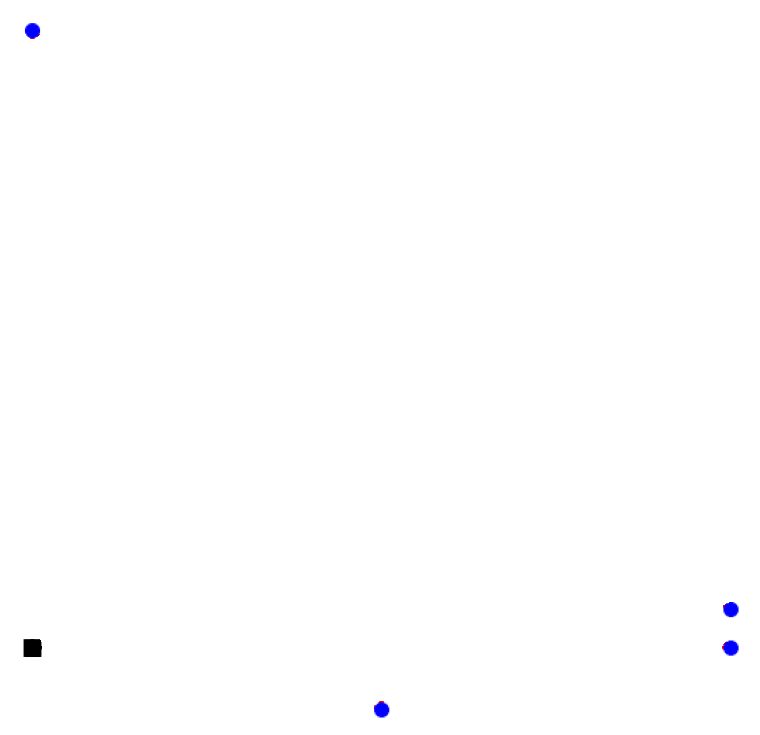
\includegraphics[width=0.37\linewidth]{poikonen_2}
			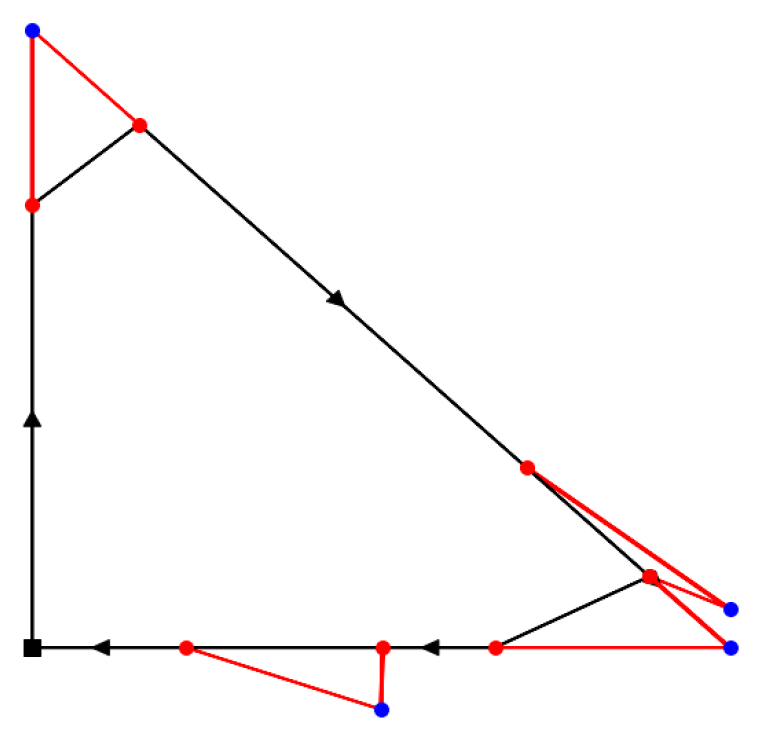
\includegraphics[width=0.37\linewidth]{poikonen_1}
		\end{center}
	\end{frame}
	
	\begin{frame}{Problem Description}
	\begin{itemize}
	    \item There is one mothership and one drone in coordination to visit a set of target graphs, whose locations are given.
	    \item For each graph $g\in\mathcal G$ the drone performs the following task:
	    \begin{enumerate}
	        \item It is launched from the current mothership location (to be determined).
	        \item It flies to the graph $g$ that has to be visited.
	        \item It traverses the required edges of graph $g$.
	        \item It returns to the current position of the mothership (to be determined).
	    \end{enumerate}
	    We assume wlog that the mothership and the drone do not need to arrive at each rendezvous location at the same time: the fastest arriving vehicle may wait for the other at the rendezvous point.
	\end{itemize}
	\end{frame}
	
	\begin{frame}{Problem Description}
	It is required to determine:
	    \begin{itemize}
	        \item The tour of the mothership starting at $orig$, deciding the different launching and rendezvous points, and returning to $dest$.
	        \item The order of visits of the target graphs followed by the drone, determining the corresponding launching and rendezvous points of the drone on each visited graph.
	        \item The tour followed by the drone on each target graph $g \in \mathcal{G}$.
	    \end{itemize}
	\end{frame}
	
	\begin{frame}{Problem Description}
	    Depending on the assumptions made on the movements of the mothership vehicle, this problem gives rise to two different versions: 
	    \begin{itemize}
	        \item The mothership vehicle can move freely on the continuous space (all terrain ground vehicle, boat on the water or aircraft vehicle), called the All terrain Mothership-Drone Routing Problem with Graphs (AMDRPG).
	        \item The mothership can move on a road network (that is, it is a normal truck or van), called the Network Mothership-Drone Routing Problem with Graphs (NMDRPG).
	    \end{itemize}
	\end{frame}
	
	\begin{frame}{Parameters of the AMDRPG}
	The known parameters of the problem are:
	\begin{itemize}
	    \item $orig$: coordinates of the point defining the origin of the mothership path (or tour).
        \item $dest$: coordinates of the point defining the destination of the mothership path (or tour).
        \item $\mathcal{G}$: set of the target graphs.\\
        \item $g = (V_g, E_g)$: set of nodes and edges of each target graph $g \in \mathcal{G}$.
        \item $\mathcal{L}(e_g)$: length of edge $e$ of graph $g \in \mathcal{G}$.
        \item $B^{e_g}, C^{e_g}$: coordinates of the endpoints of edge $e$ of graph $g \in \mathcal{G}$.
        \item $\alpha^{e_g}$: percentage of edge $e$ of graph $g \in \mathcal{G}$ that must be visited.
        \item $\alpha^g$: percentage of graph $g \in \mathcal{G}$ that must be visited.
        \item $v_D$: drone speed.
        \item $v_M$: mothership speed.
        \item $M$: big-M constant.
    \end{itemize}
	\end{frame}
	
	\begin{frame}{Initial data for the AMDRPG}
	    \begin{center}
			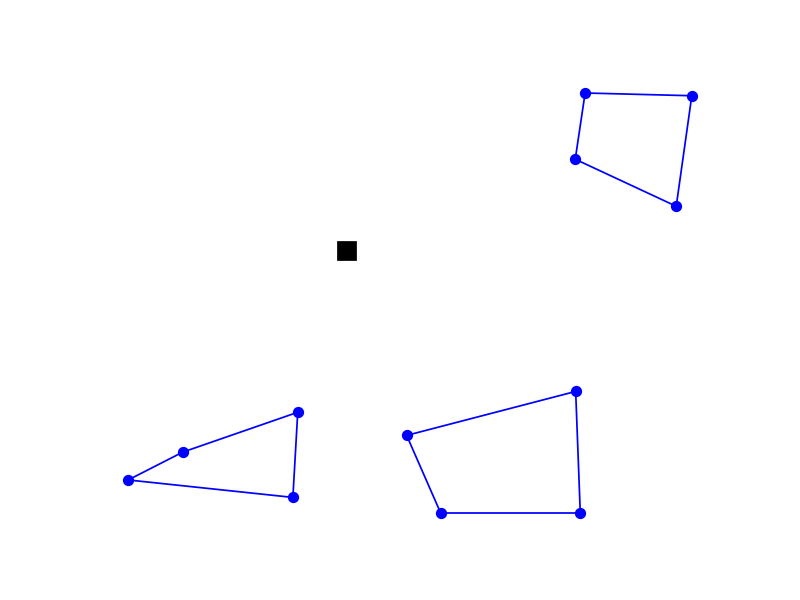
\includegraphics[width=0.7\linewidth]{PDMTZ_1}
		\end{center}
	\end{frame}
	
	\begin{frame}{Binary and Integer Decision Variables for the AMDRPG-ST}
	\begin{itemize}
	    \item $\mu^{e_g} \in \{0,1\} \:\: \forall e_g \in E_g$ ($g \in \mathcal{G}$): equal to 1 if edge $e$ of graph $g$ (or a portion of it) is visited by the drone, and  0 otherwise.
        \item $entry^{e_g} \in \{0,1\} \:\: \forall e_g \in E_g$ ($g \in \mathcal{G}$): auxiliary binary variable used for linearizing expressions.
        \item $u^{e_{g}t} \in \{0,1\} \:\: \forall e_g \in E_g$ ($g \in \mathcal{G}$) $\: \forall t \in T$: equal to 1 if the drone enters in graph $g$ by $e_g$ at stage $t$, 0 otherwise.
        \item $z^{e_{g}e^{'}_{g}} \in \{0,1\} \:\: \forall e_g, e_g' \in E_g$ ($g \in \mathcal{G}$): equal to 1 if the drone goes from $e_g$ to $e^{'}_{g}$, 0 otherwise.
        \item $v^{e_{g}t} \in \{0,1\} \:\: \forall e_g \in E_g$ ($g \in \mathcal{G}$) $\: \forall t \in T$: equal to 1 if the drone exits from graph $g$ by $e_g$ at stage $t$, 0 otherwise.
        \item $s^{e_g},\; \forall e_g \in E_g$ ($g \in \mathcal{G}$): integer non negative variable representing the order of visit of edge $e$.
    \end{itemize}
	\end{frame}
	
	\begin{frame}{Continuous Decision Variables for the AMDRPG-ST}
	\textbf{Location variables}
	\begin{itemize}
	    \item $\rho^{e_g} \in [0,1]$ and $\lambda^{e_g} \in [0,1] \:\: \forall e_g \in E_g$ ($g \in \mathcal{G}$): defining the entry and exit points on $e_g$.
        \item $\nu_\text{min}^{e_g}$ and $\nu_\text{max}^{e_g} \in [0,1] \forall e_g \in E_g$ ($g \in \mathcal{G}$): auxiliary variables used for linearizing expressions.
        \item $x_L^t \:\: \forall t \in T$: coordinates representing the point where the mothership launches the drone at stage $t$.
        \item $x_R^t \:\: \forall t \in T$: coordinates representing the point where the mothership retrieves the drone at stage $t$.
        \item $R^{e_g} \:\: \forall e_g \in E_g$ ($g \in \mathcal{G}$): coordinates representing the entry point on edge $e$ of graph $g$.
        \item $L^{e_g} \:\: \forall e_g \in E_g$ ($g \in \mathcal{G})$: coordinates representing the exit point on edge $e$ of graph $g$.
    \end{itemize}
    \end{frame}
    
    \begin{frame}{Continuous Decision Variables for the AMDRPG-ST}
    \textbf{Distance variables}
    \begin{itemize}
        \small
        \item $d_L^{e_gt} \geq 0, \:\: \forall e_g \in E_g$ ($g \in \mathcal{G}$) $\forall t \in T$: representing the distance travelled by the drone from the launching point $x_L^t$ on the mothership at stage $t$ to the first visiting point $R^{e_g}$ on $e_g$.
        \item $d^{e_ge^\prime_g} \geq 0, \:\: \forall e_g, e^\prime_g \in E_g $ ($g \in \mathcal{G}$): representing the distance travelled by the drone from the launching
        point $L^{e_g}$ on $e_g$ to the rendezvous point $R^{e^\prime_g}$ on $e^\prime_g$.
        \item $d^{e_g} \geq 0, \:\: \forall e_g \in E_g$ ($g \in \mathcal{G}$): representing the distance travelled by the drone from the rendezvous point $R^{e_g}$ to the launching point $L^{e_g}$ on $e_g$. 
        \item $d_R^{e_gt} \geq 0 \:\: \forall e_g \in E_g$ ($g \in \mathcal{G}$) $\forall t \in T$: representing the distance travelled by the drone from the last
        visiting point $L^{e_g}$ on $e_g$ to the rendezvous point $x_R^t$ on the mothership at stage $t$.
        \item $d_{LR}^t \geq 0 \:\: \forall t \in T$: representing the distance travelled by the mothership from the launching point $x_L^t$ to the rendezvous point $x_R^t$ at stage $t$.
        \item $d_{RL}^t \geq 0 \:\: \forall t \in T$: representing the distance travelled by the mothership from the rendezvous point $x_R^t$ at stage $t$ to the launching point $x_L^{(t+1)}$ at the stage $t+1$.
    \end{itemize}
	\end{frame}
	
	\begin{frame}{Distance constraints}
	    To account for the different distances among the decision variables of the model we need to set the continuous variables $d_L^{e_gt}$, $d^{e_g}$, $d^{e_ge^\prime_g}$, $d_R^{e_gt}$, $d_{RL}^t$ and $d_{LR}^t$. This can be done by means of the following constraints:
        
        \begin{align*}
        \|x_L^t- R^{e_g}\| & \leq  d_L^{e_gt},  &\quad \forall e_g:g\in \mathcal{G}, \forall t\in T \tag{DIST$_{1}$-t}, \label{eq:d1}\\
        \|R^{e_g}- L^{e_g}\| & \leq  d^{e_g},  &\quad \forall e_g:g\in \mathcal{G},\forall t\in T \tag{DIST$_{2}$-t}, \label{eq:d2}\\
        \|R^{e_g}- L^{e^\prime_g}\| & \leq  d^{e_ge^\prime_g}, &\quad \forall e_g\neq e_g'\in E_g:g\in \mathcal{G} \tag{DIST$_{3}$-t}, \label{eq:d3}\\
        \|L^{e_g}- x_R^t\| & \leq  d_R^{e_gt}, &\quad \forall e_g:g\in \mathcal{G},\forall t\in T \tag{DIST$_{4}$-t}, \label{eq:d4}\\
        \|x_R^t- x_L^{t+1}\| & \leq  d_{RL}^t, & \quad \forall t\in T, \tag{DIST$_{5}$-t} \label{eq:d5}\\
        \|x_L^t- x_R^t\| & \leq  d_{LR}^t, & \quad \forall t\in T. \tag{DIST$_{6}$-t} \label{eq:d6}\\
        \end{align*}
	\end{frame}
	
    	\begin{frame}{Visit of the graphs}
	    We have considered two modes of visit to the target graphs $g\in \mathcal{G}$ that must be represented by their corresponding constraints:
        \begin{itemize}
            \item Visiting a percentage $\alpha^{e_g}$ of each edge $e_g$ which can be modeled by:
            \begin{equation}\label{eq:alphaE}\tag{$\alpha$-E}
            |\lambda^{e_g} - \rho^{e_g}|\mu^{e_g}\geq \alpha^{e_g}, \quad \forall e_g\in E_g.
            \end{equation}
            \item Visiting a percentage $\alpha^g$ of the total length $\mathcal L(g)$ of the graph $g$ modeled by:
            \begin{equation}\label{eq:alphaG}\tag{$\alpha$-G}
            \sum_{e_g\in E_g} \mu^{e_g}|\lambda^{e_g} - \rho^{e_g}|\mathcal L(e_g) \geq \alpha^g\mathcal L(g).
            \end{equation}
            %where $\mathcal L(g)$ denotes the total length of the graph.
        \end{itemize}
	\end{frame}
	
	\begin{frame}{Visit of the graphs}
	    In both cases the corresponding constraints are nonlinear. For each edge $e_g$, we linearize the absolute value constraint \eqref{eq:alphaE} by introducing a binary variable:
        \begin{equation}\label{eq:alpha-E}\tag{$\alpha$-E}
         \mu^{e_g}|\rho^{e_g}-\lambda^{e_g}|\geq \alpha^{e_g} \Longleftrightarrow
         \left\{
         \begin{array}{ccl}
          \rho^{e_g} - \lambda^{e_g}                       & =    & \nu_\text{max}^{e_g} - \nu_\text{min}^{e_g}                                     \\
          \nu_\text{max}^{e_g}                         & \leq & 1-{\text{entry}^{e_g}}                                    \\
          \nu_\text{min}^{e_g}                      & \leq & {  \text{entry}^{e_g}},                                        \\
          \mu^{e_g}(\nu_\text{max}^{e_g} + \nu_\text{min}^{e_g} ) & \geq & \alpha^{e_g}.
          \\
         \end{array}
         \right.
        \end{equation}
        
        \noindent
        The linearization of \eqref{eq:alphaG} is similar to \eqref{eq:alphaE} and only requires changing the last inequality in \eqref{eq:alpha-E} for
        
        \begin{equation}\label{eq:alpha-G}\tag{$\alpha$-G}
        \sum_{e_g\in E_g} \mu^{e_g}(\nu_\text{max}^{e_g} + \nu_\text{min}^{e_g})\mathcal L(e_g)\geq \alpha_g\mathcal L(g).
        \end{equation}
	\end{frame}
	
	\begin{frame}{Modeling the Drone Route}
	\begin{small}

	\begin{align}
        \sum_{g\in \mathcal G}\sum_{e_g\in E_g} u^{e_gt} & = 1, &\forall t\in T \label{st:DEnt},\\%\tag{DEn}\\
        \sum_{g\in\mathcal G}\sum_{e_g\in E_g} v^{e_gt} & = 1, &\forall t\in T, \label{st:DExt}\\%\tag{DEx}\\
        \sum_{e_g\in E_g} \sum_{t\in T} u^{e_gt} & = 1, &\forall g\in\mathcal G, \label{st:DEng}\\%\tag{D
        \sum_{e_g\in E_g}\sum_{t\in T} v^{e_gt} & = 1, &\forall g\in\mathcal G, \label{st:DExg}\\%\tag{D
        \sum_{e_g\in E_g} u^{e_gt} & = \sum_{e_g\in E_g} v^{e_gt}, &\forall g\in\mathcal G, \forall t\in T, \label{st:Duv}\\%\tag{D
        \sum_{e^\prime_g\in E_g} z_g^{e^\prime_ge_g} + \sum_{t\in T} u^{e_gt} & = \mu^{e_g}, &\forall e_g\in E_g:g\in\mathcal G, \label{st:DInu}\\
        \sum_{e^\prime_g\in E_g} z_g^{e_ge^\prime_g} + \sum_{t\in T} v^{e_gt} & = \mu^{e_g}, &\forall e_g\in E_g:g\in\mathcal G. \label{st:DInv}
    \end{align}
    \end{small}
	\end{frame}
	
	\begin{frame}{Subtour elimination inside the graph}
	    \begin{small}
		To prevent the existence of subtours within each graph $g\in \mathcal G$ that the drone must visit: 
		\begin{itemize}
		\item One can add the Miller-Tucker-Zemlin constraints, given by:
    		\begin{align}
    		    s^{e_g} - s^{e^\prime_g} + |E_g|z^{e_ge^\prime_g} & \leq |E_g| - 1  , &\quad\forall e_g \neq e_g'\in E_g \tag{MTZ$_1$}, \label{MTZ1}\\
                0 & \leq s^{e_g} \leq |E_g| - 1 &\quad\forall e_g\in E_g\tag{MTZ$_2$},\label{MTZ2}
                \end{align}
        \item It is also possible to include the subtour elimination constraints:
        \begin{equation}\tag{SEC}\label{SEC}
        \sum_{e_g, e^\prime_g \in S} z_g^{e_ge^\prime_g} \leq |S| - 1, \quad \forall S\subset E_g:g\in \mathcal G.
    \end{equation}
    \end{itemize}
    \end{small}
	    
	\end{frame}
	
	\begin{frame}{Coordination constraint}
	    To ensure that the time spent by the drone to visit graph $g$ at stage $t$ is less than or equal to the time that the mothership needs to move from the launching point to the rendezvous point at stage $t$, we need to define the following coordination constraint for each $g\in \mathcal G$ and $t\in T$:

        \begin{equation}\tag{DCW-t}\label{DCW-t}
        \tiny
        \frac{1}{v_D}\left(\sum_{e_g\in E_g} u^{e_gt}d_L^{e_gt} + \sum_{e_g, e^\prime_g\in E_g}z^{e_ge^\prime_g}d^{e_ge^\prime_g} + \sum_{e_g\in E_g} \mu^{e_g}d^{e_g} + \sum_{e_g\in E_g} v^{e_gt}d_R^{e_gt}\right) \leq \frac{d_{LR}^t}{v_M} + M(1 - \sum_{e_g\in E_g} u^{e_gt}).
        \end{equation}
	\end{frame}
	
	\begin{frame}{Setting the origin and the destination}
	    Eventually, we have to impose that the tour of the mothership, together with the drone, starts from the origin $orig$ and ends at the destination $dest$. To this end, we define the following constraints:

        \begin{align*}
        x_L^0 & =  orig,  \tag{ORIG$_1$} \label{eq:O1} \\
        x_R^0 & =  orig,  \tag{ORIG$_2$} \label{eq:O2} \\
        x_L^{|\mathcal{G}|+1} & =  dest,  \tag{DEST$_1$} \label{eq:D1} \\
        x_R^{|\mathcal{G}|+1} & =  dest.  \tag{DEST$_2$} \label{eq:D2} 
        \end{align*}

	\end{frame}
	
	\begin{frame}{Formulation for the AMDRPG-ST}
	
	\begin{align*}
	    \text{min}\quad & \beta_D(\sum_{g\in\mathcal G}\sum_{e_g\in E_g}\sum_{t\in T} (u^{e_gt}d_L^{e_gt} + v^{e_gt}d_R^{e_gt}) + \sum_{g\in\mathcal G}\sum_{e_g\in E_g} \mu^{e_g}d^{e_g} + \\
	    + & \sum_{g\in\mathcal G}\sum_{e_g,e^\prime_g\in E_g}z^{e_ge^\prime_g}d^{e_ge^\prime_g}) + \beta_M\sum_{t\in T} (d_{RL}^t + d_{LR}^t) \\
	    \text{s.t.}\quad & \eqref{st:DEnt}-\eqref{st:DInv}, \\
	    & \eqref{MTZ1} - \eqref{MTZ2} \text{ or } \eqref{SEC}, \\
	    & \eqref{eq:alpha-E} \text{ or } \eqref{eq:alpha-G}, \\
	    & \eqref{DCW-t}, \\
	    & \eqref{eq:d1}-\eqref{eq:d6}, \\
	    & \eqref{eq:O1}-\eqref{eq:D2}.
	\end{align*}
% 	\begin{mini*}|s|
%          {}{\sum_{g\in\mathcal G}\sum_{e_g\in E_g}\sum_{t\in T} (u^{e_gt}d_L^{e_gt} + v^{e_gt}d_R^{e_gt}) + \sum_{g\in\mathcal G}\sum_{e_g\in E_g} \mu^{e_g}d^{e_g} +
%          \breakObjective{\sum_{g\in\mathcal G}\sum_{e_g,e^\prime_g\in E_g}z^{e_ge^\prime_g}d^{e_ge^\prime_g} + \sum_{t\in T} (d_{RL}^t + d_{LR}^t)}}{}{} \label{AMDRPG-ST} \tag{AMDRPG-ST}
%          \addConstraint{\eqref{st:DEnt}-\eqref{st:DInv}}{}{}
%          \addConstraint{\eqref{MTZ1} - \eqref{MTZ2} \text{ or } \eqref{SEC} }{}{}
%          \addConstraint{\eqref{eq:alpha-E} \text{ or } \eqref{eq:alpha-G}}{}{}
%          \addConstraint{\eqref{DCW-t}}{}{}
%          \addConstraint{\eqref{eq:d1}-\eqref{eq:d6}}{}{}
%          \addConstraint{\eqref{eq:O1}-\eqref{eq:D2}}.{}{}
%     \end{mini*}
	    
	\end{frame}
	
	\begin{frame}{Alternative formulations based on enforcing connectivity}
	    In this family of formulations we replace the variables $u^{\cdot t}, v^{\cdot t}$ and constraints that model the tour using stages, namely (1)-(7), by constraints that ensure connectivity.
	    
	    \bigskip
	    
	    We will distinguish two different approaches:
    	\begin{itemize}
    		\item Using Miller-Tucker-Zemlin compact formulation.
    		\item Using the known subtour elimination constraints.
    	\end{itemize}
	\end{frame}
	
	\begin{frame}{\large Binary and Integer Decision Variables for the AMDRPG-MTZ}
	\begin{itemize}
	    \small
	    \item $\mu^{e_g} \in \{0,1\} \:\: \forall e_g \in E_g$ ($g \in \mathcal{G}$): equal to 1 if edge $e$ of graph $g$ (or a portion of it) is visited by the drone, and 0 otherwise.
        \item $entry^{e_g} \in \{0,1\} \:\: \forall e_g \in E_g$ ($g \in \mathcal{G}$): auxiliary binary variables for linearization.
        \item $u^{e_{g}} \in \{0,1\} \:\: \forall e_g \in E_g$ ($g \in \mathcal{G}$): equal to 1 if the drone enters in graph $g$ by $e_g$, 0 otherwise.
        \item $z^{e_{g}e^{'}_{g}} \in \{0,1\} \:\: \forall e_g, e_g' \in E_g$ ($g \in \mathcal{G}$): equal to 1 if the drone goes from $e_g$ to $e^{'}_{g}$, 0 otherwise.
        \item $v^{e_{g}} \in \{0,1\} \:\: \forall e_g \in E_g$ ($g \in \mathcal{G}$): equal to 1 if the drone exits from graph $g$ by $e_g$, 0 otherwise.
        \item \textcolor{red}{$w^{gg'} \in \{0,1\} \:\:\ \forall g,g' \in \mathcal{G}$: equal to 1 if the mothership moves from $x_R^g$ to $x_L^{g^'}$, 0 otherwise.}
        \item $s^{e_g} \:\: \forall e_g \in E_g$ ($g \in \mathcal{G}$): integer non negative variables representing the order of visit of edge $e$ of graph $g$.
    \end{itemize}
	\end{frame}
	
	\begin{frame}{Continuous Decision Variables for the AMDRPG-MTZ}
	\textbf{Location variables}
	\begin{itemize}
        \item $\rho^{e_g} \in [0,1]$ and $\lambda^{e_g} \in [0,1] \:\: \forall e_g \in E_g$ ($g \in \mathcal{G}$): defining the entry and exit points on $e_g$.
        \item $\nu_\text{min}^{e_g}$ and $\nu_\text{max}^{e_g} \in [0,1] \:\: \forall e_g \in E_g$ ($g \in \mathcal{G}$): auxiliary variables for linearization.
        \item $x_L^g \:\: \forall g \in \mathcal{G}$: pairs of coordinates representing the point where the mothership launches the drone to visit graph $g$.
        \item $x_R^g \:\: \forall g \in \mathcal{G}$: pairs of coordinates representing the point where the mothership retrieves the drone after visit graph $g$.
        \item $R^{e_g} \:\: \forall e_g \in E_g$ ($g \in \mathcal{G}$): coordinates representing the entry point on edge $e$ of graph $g$.
        \item $L^{e_g} \:\: \forall e_g \in E_g$ ($g \in \mathcal{G}$): coordinates representing the exit point on edge $e$ of graph $g$.
    \end{itemize}
    \end{frame}
    
    \begin{frame}{Continuous Decision Variables for the AMDRPG-MTZ}
    \textbf{Distance variables}
    \begin{itemize}
        \footnotesize
        \item $d_L^{e_g} \geq 0 \:\: \forall e_g \in E_g$ ($g \in \mathcal{G}$): representing the distance travelled by the drone from the launching point 
         on the mothership  $x_L^g$ to the first visiting point $R^{e_g}$ on edge $e_g$.
        \item $d^{e_ge^\prime_g} \geq 0 \:\: \forall e_g, e^\prime_g \in E_g $ ($g \in \mathcal{G}$): representing the distance travelled by the drone from launching point $L^{e_g}$ on $e_g$ to the rendezvous point $R^{e^\prime_g}$ on $e^\prime_g$.
        \item $d^{e_g} \geq 0 \:\: \forall e_g \in E_g$ ($g \in \mathcal{G}$): representing the distance travelled by the drone from the rendezvous point
$R^{e_g}$ to the launching point $L^{e_g}$ on $e_g$. 
        \item $d_R^{e_g} \geq 0 \:\: \forall e_g \in E_g$ ($g \in \mathcal{G}$): representing the distance travelled by the drone from the last visiting point
 $L^{e_g}$ on $e_g$ to the rendezvous point $x_R^g$ on the mothership.
        \item $d_{LR}^g \geq 0 \:\: \forall g \in \mathcal{G}$: representing the distance travelled by the mothership from the launching point
 $x_L^g$ to the rendezvous point $x_R^g$ while the drone is visiting $g$.
        \item $d_{RL}^{gg_\prime} \geq 0 \:\: \forall g, g^{'} \in \mathcal{G}$: representing the distance travelled by the mothership from the 
rendezvous point $x_R^g$ for graph $g$ to the launching point $x_L^{g\prime}$ for graph $g\prime$.
    \end{itemize}
	\end{frame}
	
	\begin{frame}{Distance Constraints}
	    \begin{align*}
        \|x_L^g- R^{e_g}\| &\leq d_L^{e_g},&\quad \forall e_g:g\in\mathcal G, \tag{DIST$_{1}$-g} \label{eq:d1g}\\
        \|R^{e_g}- L^{e_g}\| &\leq d^{e_g},&\quad \forall e_g:g\in\mathcal G, \tag{DIST$_{2}$-g}\\
        \|R^{e_g}- L^{e^\prime_g}\| &\leq d^{e_ge^\prime_g},&\quad \forall e_g\neq e'_g:g\in\mathcal G, \tag{DIST$_{3}$-g}\\
         \|L^{e_g}- x_R^g\| &\leq d_R^{e_g},&\quad \forall e_g:g\in\mathcal G, \tag{DIST$_{4}$-g}\\
        \|x_R^g- x_L^{g'}\| &\leq d^{gg'}_{RL},& \quad \forall g,g'\in\mathcal G, \tag{DIST$_{5}$-g}\\
        \|x_L^g- x_R^g\| &\leq d^g_{LR},& \quad \forall g\in\mathcal G. \tag{DIST$_{6}$-g} \label{eq:d6g}\\
        \end{align*}
	\end{frame}
	
	
	\begin{frame}{Modeling the Drone Route}
	We can model the route that the drone follows in each particular graph $g\in \mathcal G$:
	\begin{align}
        \sum_{e_g\in E_g} u^{e_g} & = 1, & \quad\forall g \in \mathcal G, \label{DEnt2}\\%\tag{DEn}\\
        \sum_{e_g\in E_g} v^{e_g} & = 1, & \quad\forall g \in \mathcal G, \label{DExt}\\%\tag{DEx}\\
        \sum_{e^\prime_g\in E_g} z^{e_g'e_g} + u^{e_g} & = \mu^{e_g}, &\quad\forall e_g\in E_g:g\in\mathcal G, \label{DInu}\\
        \sum_{e^\prime_g\in E_g} z^{e_ge_g'} + v^{e_g} & = \mu^{e_g}, &\quad\forall e_g\in E_g:g\in\mathcal G. \label{DInv2}
    \end{align}
	\end{frame}
	
	\begin{frame}{Modeling the Mothership Route}
	On the other hand, to model the tour followed by the mothership, we have to include the following new constraints:
		{\color{red}
	    \begin{align}
	        \small
            \sum_{g\in\mathcal G} w^{g0} & = 0, \label{TOrig}\\
            \sum_{g'\in\mathcal G} w^{(n_G+1) g'} & = 0, \label{TDest}\\
            \sum_{g'\in\mathcal G\setminus\{g\}} w^{gg'} & = 1, \label{TExt} &\quad\forall g\in \mathcal G,\\
            \sum_{g\in\mathcal G\setminus\{g'\}} w^{gg'} & = 1, &\quad\forall g'\in \mathcal G,\label{TEnt}\\
            s_g - s_{g'} + |\mathcal G|w^{gg'} & \leq |\mathcal G| - 1  , &\quad\forall g \neq g', \tag{MTZ$_3$} \label{MTZ3}\\
            0 & \leq s_g \leq |\mathcal G| - 1 &\quad\forall g\in \mathcal G,\tag{MTZ$_4$}\label{MTZ4}\\
            s_0 & = 0, \tag{MTZ$_5$}\label{MTZ5}\\
            s_{n_G+1}&=n_G+1. \tag{MTZ$_6$}\label{MTZ6}
        \end{align}}
	\end{frame}
	
	\begin{frame}{Coordination constraint}
	    Again, we need to be sure that the time spent by the drone to visit the graph $g$ is less than or equal to the time that the mothership needs to move from the launching point to the rendezvous point associated to this graph $g$. Hence, by using the same argument, as the one used in \eqref{DCW-t}, we define for each $g\in \mathcal G$:
        \begin{equation}
        \footnotesize
         \frac{1}{v_D}\left(\sum_{e_g\in E_g} u^{e_g}d_L^{e_g} + \sum_{e_g, e^\prime_g\in E_g}z^{e_ge^\prime_g}d^{e_ge^\prime_g} + \sum_{e_g\in E_g} \mu^{e_g} d^{e_g} + \sum_{e_g\in E_g}v^{e_g}d_R^{e_g}\right)\leq \frac{d_{LR}^{g}}{v_M}, \quad\forall g\in\mathcal G.\label{DCW-g}\tag{DCW-g}
        \end{equation}

	\end{frame}
	
	\begin{frame}{Formulation for the AMDRPG-MTZ (resp. SEC)}
	\begin{footnotesize}
	\begin{align*}
	    \text{min}\quad &\beta_D(\sum_{g\in\mathcal G}\sum_{e_g\in E_g} (u^{e_g}d_L^{e_g} + v^{e_g}d_R^{e_g}) + \sum_{g\in\mathcal G}\sum_{e_g\in E_g} \mu^{e_g} d^{e_g} + \\
	    + & \sum_{g\in\mathcal G}\sum_{e_g,e^\prime_g\in E_g}z^{e_ge^\prime_g}d^{e_ge^\prime_g}) + \beta_M(\sum_{g\in\mathcal G} d_{LR}^g + \sum_{g,g'\in \mathcal G}d_{RL}^{gg'}w^{gg'}) \\
	    \text{s.t.}\quad & \eqref{DEnt2}-\eqref{TEnt}, \\
	    & \eqref{MTZ1} - \eqref{MTZ2} \text{ or } \eqref{SEC}, \\
	    & \eqref{MTZ3} - \eqref{MTZ6}, \\
	    & \eqref{eq:alpha-E} \text{ or } \eqref{eq:alpha-G}, \\
	    & \eqref{DCW-g}, \\
	    & \eqref{eq:d1g}-\eqref{eq:d6g}, \\
	    & \eqref{eq:O1}-\eqref{eq:D2}.
	\end{align*}
	\end{footnotesize}
	The formulation above can be slightly modified replacing constraints $\eqref{MTZ3} - \eqref{MTZ6}$ by
    \begin{equation}\label{SEC-graph}
    \sum_{g,g'\in \mathcal G} w^{gg'} \le |S|-1, \quad \forall S\subseteq \{1,\ldots, |\mathcal G|\}.
    \end{equation}

	\end{frame}
	
	\begin{frame}{Example 1}
    \begin{figure}
        \centering
        \subfigure{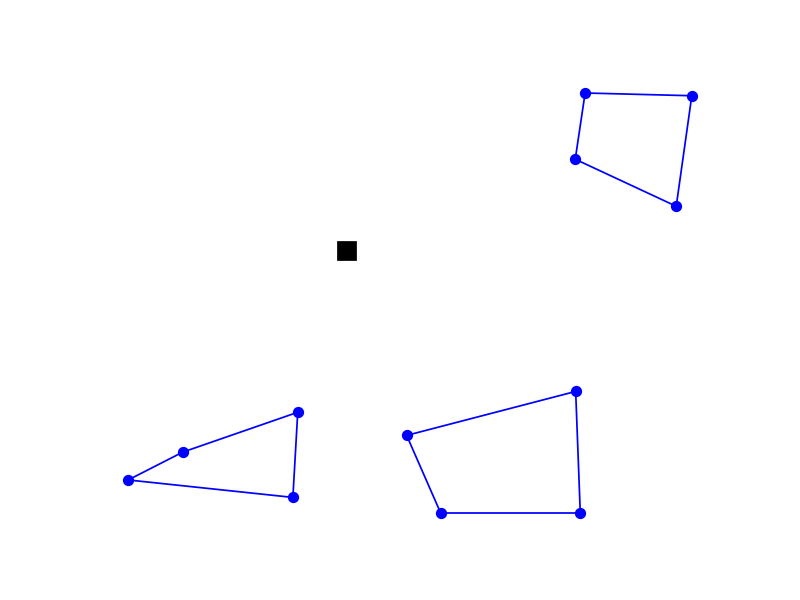
\includegraphics[width=0.28\textwidth]{PDMTZ_1.png}} 
        \subfigure{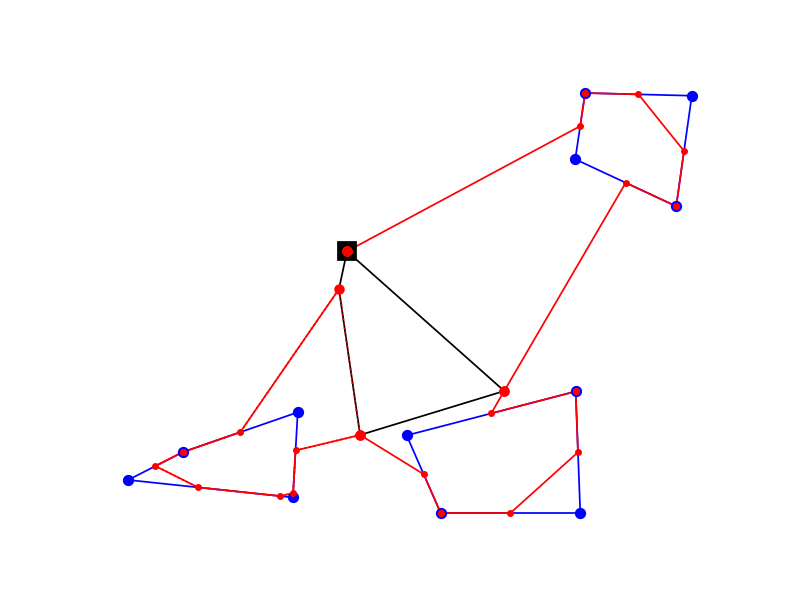
\includegraphics[width=0.28\textwidth]{PDMTZ_e.png}} 
        \subfigure{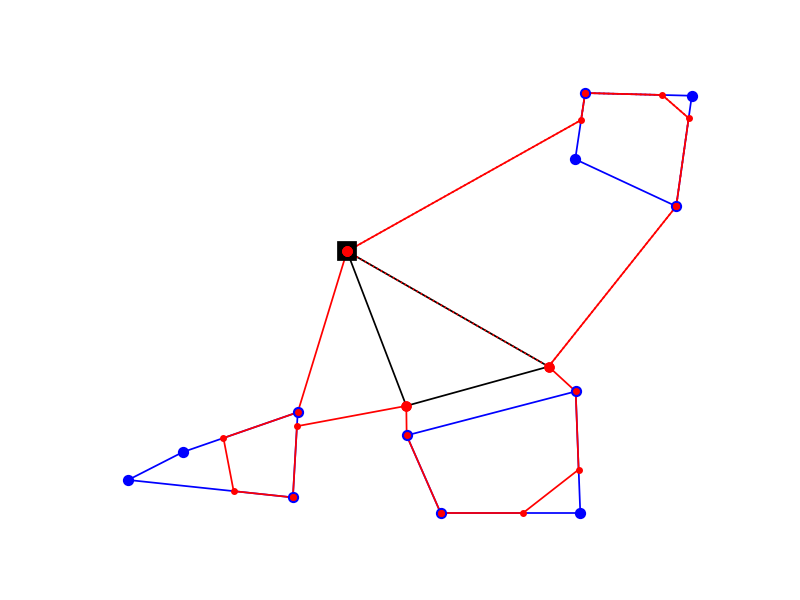
\includegraphics[width=0.28\textwidth]{PDMTZ_g.png}}
        \caption{(a) Origin and target graphs, (b) Visit of $\alpha^{e_g}\%$ of each edge, (c) Visit of $\alpha_g\%$ of each graph.}
        \label{fig:illustrative}
    \end{figure}	
    \end{frame}
    
    \begin{frame}{Example 2: Percentage of each edge}
    	\begin{center}
			\animategraphics[controls, width = 0.7\linewidth]{3}{gif_mdrpg_alphae/}{0}{20}
		\end{center}
    \end{frame}

    \begin{frame}{Example 3: Percentage of each graph}
    	\begin{center}
			\animategraphics[controls, width = 0.7\linewidth]{3}{gif_mdrpg_alphag/}{0}{20}
		\end{center}
    \end{frame}
	
	\begin{frame}{Matheuristic for the AMDRPG}
	   \textbf{Pseudo-code of this algorithm:}
	   \begin{itemize} 
            \item[STEP 1] (Centroids of the graphs)\\
            - Let $orig$ be the origin/destination of the mothership tour. \\ %(orange point with label $0$ in Figure \ref{fig:example} [a]).\\
            For each graph $g \in \mathcal G$:\\
            - identify its centroid $c_g$ and consider its neighborhood defined as the circle $\rho(c_g,2)$ centered at $c_g$ and with radius 2. %(red points in Figure \ref{fig:example} [a]).
            \item[STEP 2] (Order of visit of the graphs)
            Determine an order of visit for the graphs in $\mathcal{G}$ by solving the XPPN of the mothership over the set of the neighborhoods associated with the centroids of those graphs. %(blue tour 0, 1, 2, 3, 4, 0 in Figure  \ref{fig:example} [a]).\\
        \end{itemize}
    \end{frame}
    
    \begin{frame}{Matheuristic for the AMDRPG}
    \textbf{Pseudo-code of this algorithm:}
    \begin{itemize}
        \small
            \item[STEP 3] (Determining the location of launching/rendezvous points)
            Let $\bar{w}_{gg^{'}}, \: \forall g,g^{'} \in \mathcal G$ be the optimal values of the variables $w_{gg^{'}}$ generated by STEP 2.\\
            Following this order of visit, set the launching point for the first graph as the depot, then solve the resulting (MDRPG) limited to the first graph.\\
            Repeat the same procedure for the remaining graphs to be visited, by solving \AMD\xspace on one single graph each time, by fixing as launching point of the current graph the rendezvous point of the previous graph.
            
            \item [STEP 4] (Solution update) 
            Let $\bar{z}$ be the solution obtained by STEP 3, consisting of the tour of the drone on each target,  %(Figure \ref{fig:example} [b])
            and let $\bar{x}_{L}^{g}$, $\bar{x}_{R}^{g} \:\: \forall g \in \mathcal G$ be the associated launching/rendezvous points %(green and blue points in Figure \ref{fig:example} [b]).\\
            Solve the model (MDRPG) with these launching/rendezvous points but leaving free the $w_{gg^{'}} \:\:\ \forall g,g^{'} \in \mathcal G$ variables and providing to the solver $\bar{z}$ as initial partial solution.
            \item [STEP 5]
            Let $\hat{z}$ be the updated solution obtained by STEP 4 %(see Figure \ref{fig:example} [b] for this illustrative example) 
            and $\hat{w}_{gg^{'}}$ the associated order of visit of the graphs.\\
            If the $\hat{w}_{gg^{'}} \neq \bar{w}_{gg^{'}}$ repeat from STEP 3, otherwise stop.
            \end{itemize}
	\end{frame}

    \begin{frame}{Example of the Matheuristic}	
		\begin{figure}%
    		\hspace{-2.5cm}
        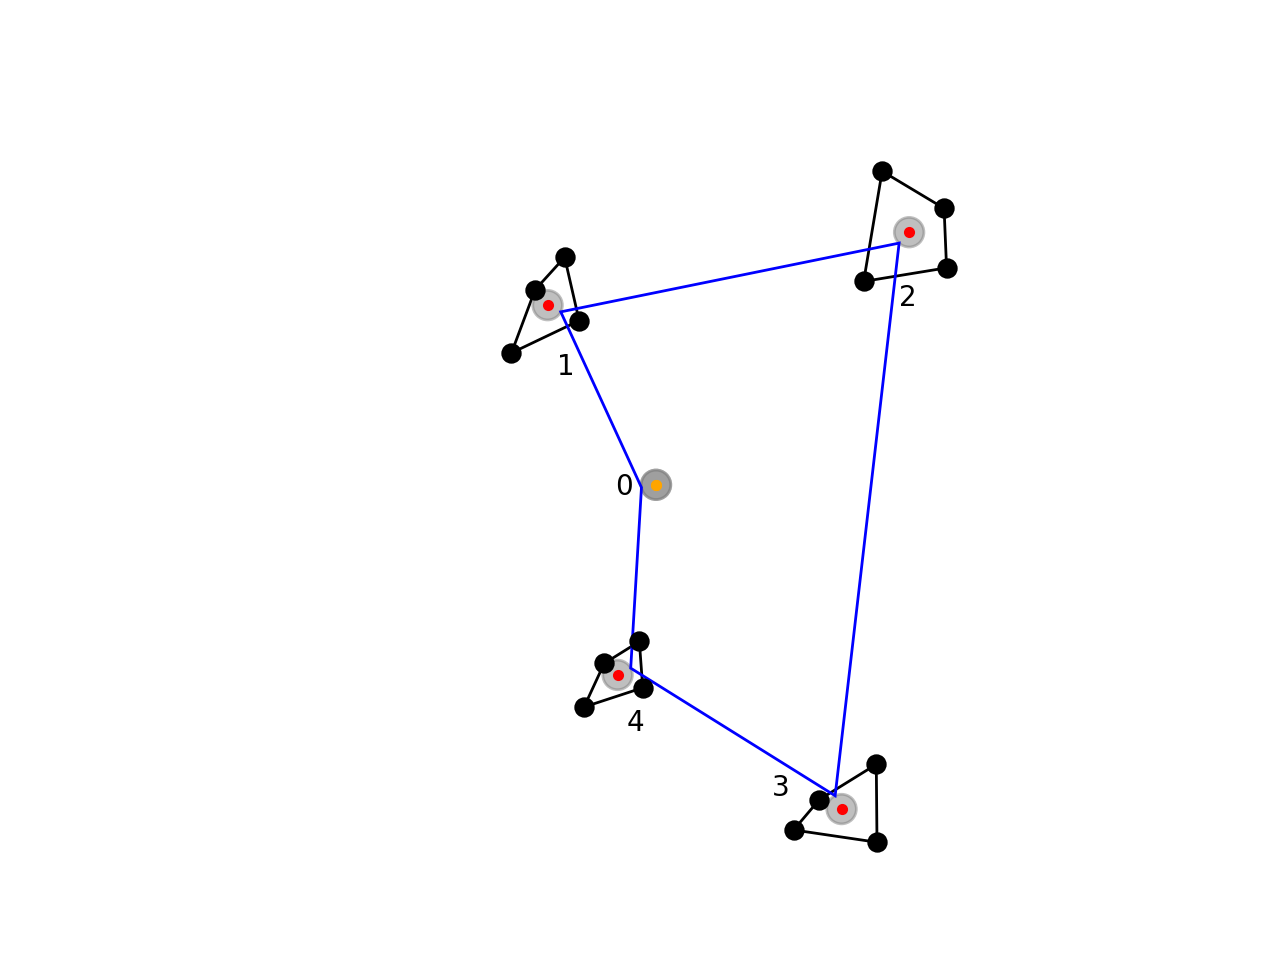
\includegraphics[width=7cm]{step0}\hspace{-1.5cm}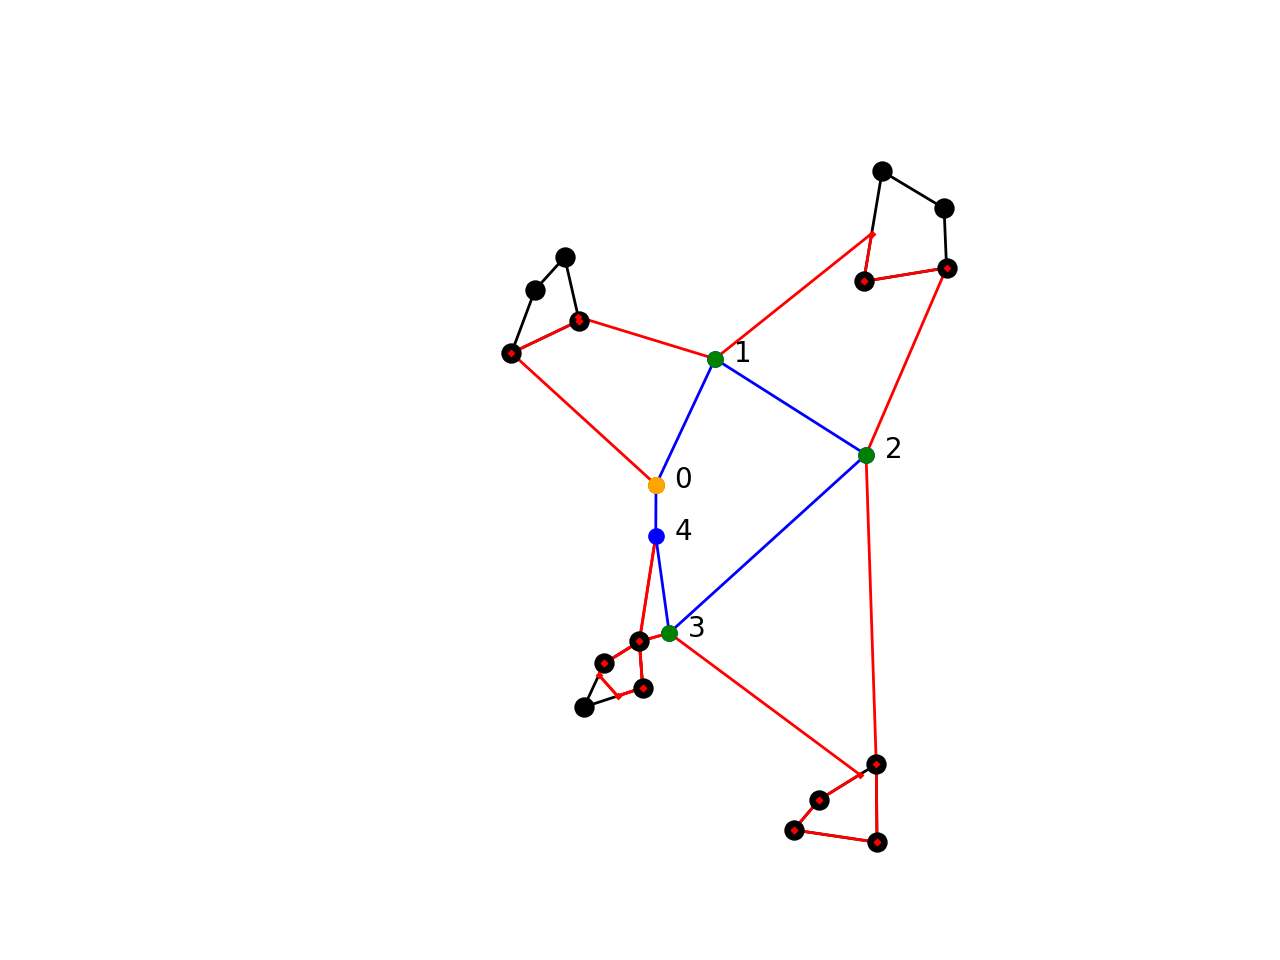
\includegraphics[width=7cm]{step1}%
        \caption{Illustrative Example}%
        \label{fig:example}%
    	\end{figure}
    \end{frame}
    
    \begin{frame}{Computational Experiments: Data Generation}
        We consider two typology of planar graphs:
        \begin{itemize}
            \item Grid graphs
            \item Delaunay triangulation (computed by using the Python class scipy.spatial.Delaunay)
        \end{itemize}
    \end{frame}
    
%    \begin{frame}{Computational Experiments: Grid Generation}
%    To simulate graphs that are similar to the one found in a road network, we design grid graphs following these steps:
%    \begin{enumerate}
%        \item We consider a square of side 100 units that we divide in subsquares of side 5 and we randomly select among them the locations for each graph.
%        \item Each subsquare of side 5 selected is further partitioned in subsquares of side $\frac{5}{n}$ where $n$ is the cardinality of the set of nodes of the graph to build.
%        \item Two opposite corner subsquares are considered and one point inside each of them is randomly selected.
%        \item A grid of $n$ points is identified by locating $\frac{n}{m}$ equally spaced points on the two sides square rectangle whose diagonal joins these two points is built, where $m$ is randomly selected in the set of divisors of the number of points of the graph.
%    \end{enumerate}
%        
%    \end{frame}
%	
%	\begin{frame}{Computational Experiments: Grid Generation}
%    To simulate graphs that are similar to the one found in a road network, we design grid graphs following these steps:
%    \begin{enumerate}
%        \setcounter{enumi}{4}
%        \item The links of the graphs connect each point to its adjacent ones lying on the same side and with the one located on the opposite side of the square.
%        \item Let $width_x$ and $width_y$ be the lengths of these edges. In order to perturb the coordinates of these points, we randomly add a value, ranging between $-\frac{width_x}{3}$ and $\frac{width_x}{3}$ to the $x$ coordinate and between $-\frac{width_y}{3}$ and $\frac{width_y}{3}$ to the $y$ coordinate, always imposing that the perturbed point still belongs to the square.
%        \item The resulting grid graph is obtained connecting the same pairs of points but with perturbed coordinates.
%    \end{enumerate}
%        
%    \end{frame}
	
	\begin{frame}{Computational Experiments: Grid Generation}
        \begin{figure}[h!]
        \begin{center}
         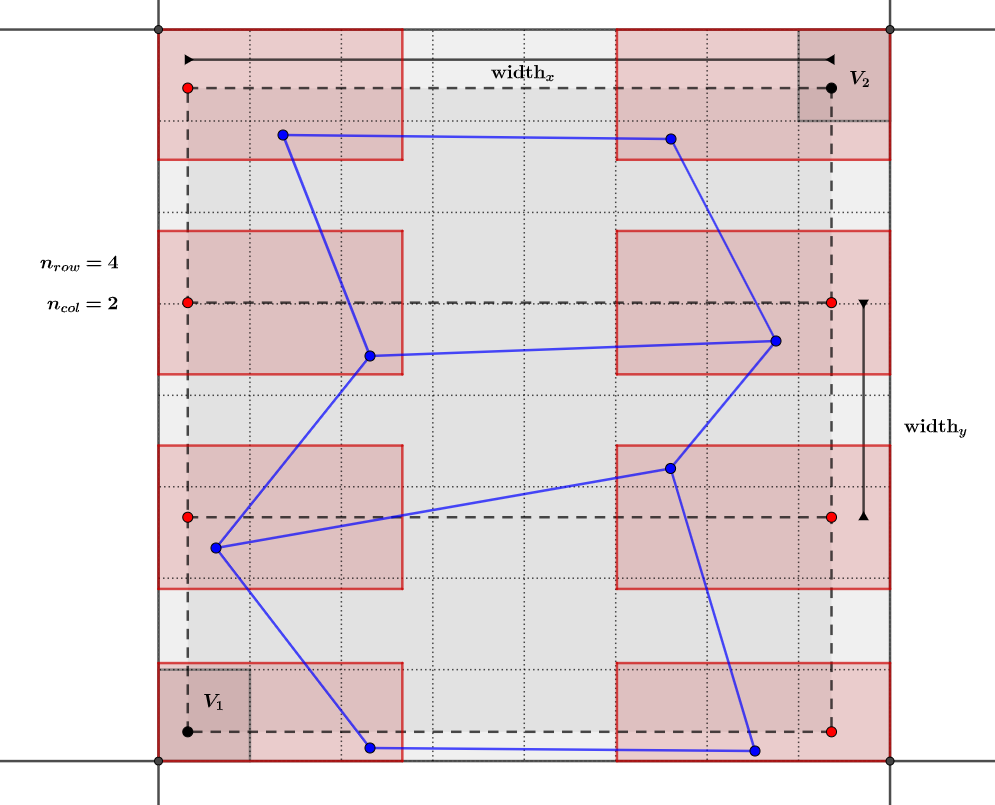
\includegraphics[width=0.6\linewidth]{Grid_generation_2.png}
        \end{center}
        \caption{Example of generation of a grid graph}
        \label{fig:fig1}
        \end{figure}
 
	\end{frame}
	
	\begin{frame}{Experiment 1: Comparing Gurobi and Cplex}
	    We generate five instances with a number $|\mathcal G|= 10$ of target graphs:
	    \begin{itemize}
	        \item 3 graphs with 4 nodes, 3 graphs with 6 nodes, 3 graphs with 8 nodes and 1 graph with 10 nodes.
	        \item $v_D= 2v_M$.
	        \item $80\%$ of each target must be visited by the drone.
	    \end{itemize}
	    
	    The experiment consists on:
	    \begin{itemize}
	        \item Running the three formulations proposed for the (AMDRPG): Stages, MTZ and SEC.
	        \item Using two commercial solvers, Cplex 12.8 and Gurobi 9.03.
	        \item Time Limit: 1 hour.
	    \end{itemize}
	\end{frame}
	
	\begin{frame}{Experiment 1: Results}
		\renewcommand{\arraystretch}{0.7}
        \begin{table}[!h]
        \caption{Comparison between formulations for grid instances}
        \centering
        \footnotesize
        \begin{tabular}{c | c c | c c | c c}
        \hline\hline
        \textbf{Gap} & \multicolumn{2}{c}{Average} &  \multicolumn{2}{c}{Min} &  \multicolumn{2}{c}{Max} \\
         % \hline
        \textbf{Solver} &Cplex &Gurobi &Cplex &Gurobi  &Cplex &Gurobi \\
        \hline
        \textbf{Formulation} & & & & & &\\
        Stages & 0,87 &	0,87 &	0,85 &	0,84 &	0,88 &	0,88\\
        MTZ	 & 0,66 &	0,62 &	0,59 &	0,58 &	0,72 &	0,65\\
        SEC	& 0,65 &	0,61 &	0,59 &	0,57 &	0,70 &	0,64\\
            \hline
        \end{tabular}
        \label{table:tab1}
        \end{table}
        
        \renewcommand{\arraystretch}{0.7}
        \begin{table}[!h]
        \caption{Comparison between formulations for Delauney instances}
        \centering
        \footnotesize
        \begin{tabular}{c | c c | c c | c c}
        \hline\hline
        \textbf{Gap} & \multicolumn{2}{c}{Average} &  \multicolumn{2}{c}{Min} &  \multicolumn{2}{c}{Max} \\
         % \hline
        \textbf{Solver} &Cplex &Gurobi &Cplex &Gurobi  &Cplex &Gurobi \\
        \hline
        \textbf{Formulation} & & & & & &\\
        Stages &	0,91 &	0,91 &	0,90 &	0,89 &	0,93 &	0,93\\
        MTZ	& 0,78 &	0,74 &	0,74 &	0,70 &	0,82 &	0,79\\
        SEC	& 0,77 &	0,75 &	0,73 &	0,69 &	0,82 &	0,81\\
            \hline
        \end{tabular}
        \label{table:tab2}
        \end{table}
	    
	\end{frame}
	
	\begin{frame}{Experiment 2: Testing the performance of the Matheuristic}
	
    We generate five instances for each number $|\mathcal G|\in\{5, 10, 15, 20\}$ of target graphs:
    \begin{itemize}
        \item The same percentage of graphs ($20\%$) has respectively 4, 6, 8, 10 and 12 nodes.
        \item $v_D= 3v_M$.
        \item $\alpha^g$ and $\alpha^{e_g}$ randomly generated in $[0, 1]$.
    \end{itemize}
    
    The experiment consists on:
    \begin{itemize}
        \item Running the MTZ formulation for (AMDRPG) with and without initial solution provided by the matheuristic.
        \item Using Gurobi 9.03.
        \item Time Limit: 2 hours.
    \end{itemize}
	    
	\end{frame}
	
	\begin{frame}{Experiment 2: Results}
    \renewcommand{\arraystretch}{0.7}
    \begin{table}[!h]
    \caption{Comparison between exact resolution with and without initialization}
    \centering
    \footnotesize
    \begin{tabular}{c c | c c c | c c c}
    \hline
     &  & \multicolumn{3}{c}{\textbf{Grid}} &  \multicolumn{3}{c}{\textbf{Delauney}} \\
    \hline
     List &  $\%$  & Gap (i) & Time$\_$h & Gap (wi)  & Gap (i) & Time$\_$h & Gap (wi)\\
    \hline
    \multirow{}{}{0} & e & 0.72 & 105.12 & 0.73 & 0.78 & 154.92 & 0.74\\
    & g & 0.55 & 58.92 & 0.54 & 0.62 & 92.64 & 0.67\\
    \hline
    \multirow{}{}{1} & e & 0.76 & 241.99 & 0.76 & 0.80 & 314.69 & 0.79\\
    & g & 0.71 & 182.61 & 0.70 & 0.74 & 353.04 & 0.75\\
    \hline
    \multirow{}{}{2} & e & 0.76 & 367.69 & 0.76 & 0.80 & 447.61 & 0.80 \\
    & g & 0.71 & 326.49 & 0.72 & 0.76 & 429.16 & 0.76\\
    \hline
    \multirow{}{}{3} & e & 0.75 & 481.68 & 0.74 & 0.80 & 514.98 & 0.76^*\\
    & g & 0.71 & 492.27 & 0.70 & 0.77 & 582.90 & 0.77\\
        \hline
    \end{tabular}
    \label{table:tab4}
    \end{table}
	\end{frame}
	
	\begin{frame}
	    \begin{figure}
	        \centering
            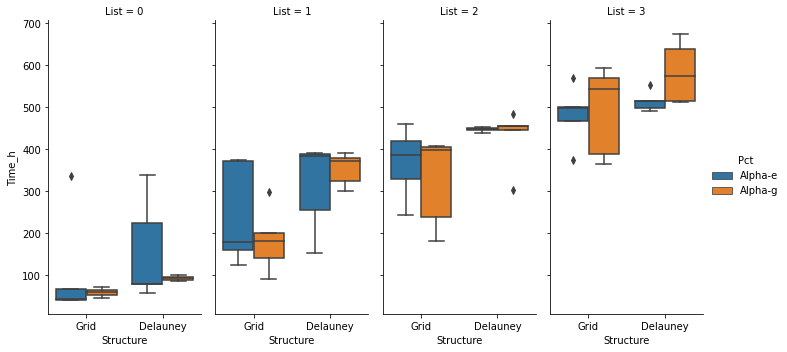
\includegraphics[width=1\linewidth]{time_h.png}
            \caption{Matheuristic running time}
            \label{fig:1}
	    \end{figure}
	\end{frame}
	\begin{frame}
	    \begin{figure}
    	    \centering
            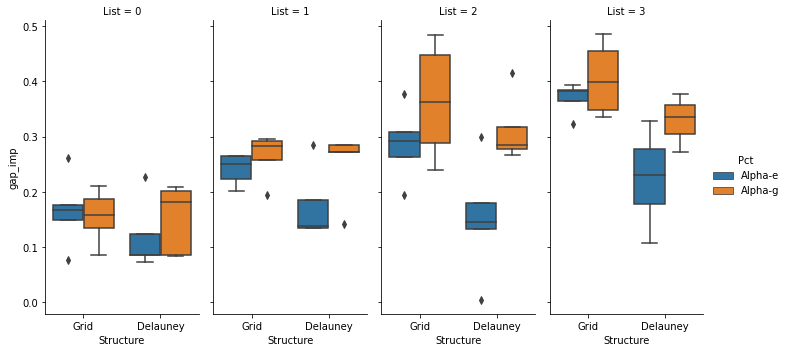
\includegraphics[width=1\linewidth]{improved_gap.png}
            \caption{Matheuristic improved gap}
	    \end{figure}
	\end{frame}
%	\begin{frame}
%	    \begin{figure}
%            \centering
%            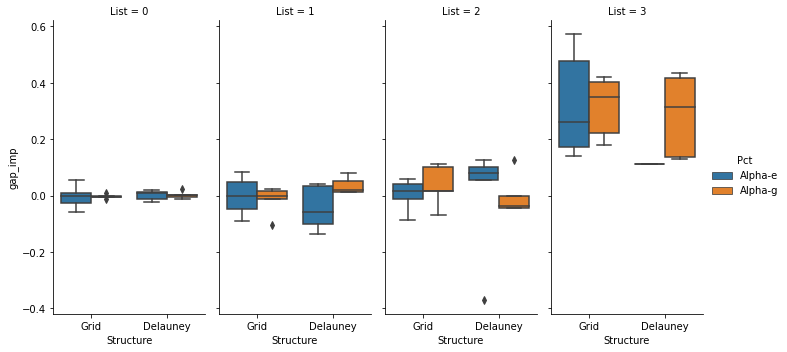
\includegraphics[width=1\linewidth]{differencewithwithout.png}
%            \caption{Improved gap of MTZ formulation with and without initialization}
%            \label{fig:3}
%        \end{figure}
%	\end{frame}
	
	\begin{frame}{Conclusions}
		\begin{itemize}
			\item Coordination problem that arises between a mothership vehicle and a drone that must adjust their routes to minimize travel distances while visiting a set of targets modeled by graphs.
			\item Exact formulations for different versions of the problem depending on the constraints imposed to the mothership movement.
			\item The considered problem is rather hard and only small to medium size problems can be  solved to optimality.
			\item Matheuristic algorithm that provides acceptable feasible solutions in short computing time.
		\end{itemize}
	
	\end{frame}

    \begin{frame}{Acknowledgements}
        This research has been partially supported by Spanish Ministry of Education and Science/FEDER grant number  MTM2016-74983-C02-(01-02), and projects FEDER-US-1256951, Junta de Andaluc\'ia P18-FR-1422, CEI-3-FQM331 and  \textit{NetmeetData}: Ayudas Fundaci\'on BBVA a equipos de investigaci\'on cient\'ifica 2019.
    \end{frame}
    
	\begin{frame}
	    \bigskip
	    \begin{figure}
	        \centering
	        
\includegraphics[width=0.7\linewidth]{thank.jpg}
	    \end{figure}
	\end{frame}
	
	
	\begin{frame}[allowframebreaks]
		\frametitle{Bibliography}
		\nocite{*}

		\bibliographystyle{plain}
		\bibliography{bibliography2}
	\end{frame}
	
	
	
	
	
	
	
	
	
	
	
	
	
	
	
	
	
	
	
\end{document}
